% -*- root: main.tex -*-
The goal of our research is to develop an automatic way to detect design and requirement \SATD comments. To do so, we first manually classify a large number of comments identifying which ones are \SATD. With the resulting dataset, we train the \revised{maximum entropy classifier}{R2-11} to identify design and requirement \SATD (RQ1). To better understand what words indicate \SATD, we inspect the features used by the \revised{maximum entropy classifier}{R2-11} to identify the detected \SATD. These features are words that are frequently found in comments with technical debt. We present the 10 most common words that indicate design and requirement \SATD (RQ2). Since the manual classification required to create our training dataset is expensive, ideally we would like to achieve maximum performance with the least amount of training data. Therefore, we investigate how variations in the size of training data affects the performance of our classification (RQ3). We detail the motivation, approach and present the results of each of our research questions in the remainder of this section. 

\begin{figure*}[!thb]
  \centering
  \subfigure[Design Debt]{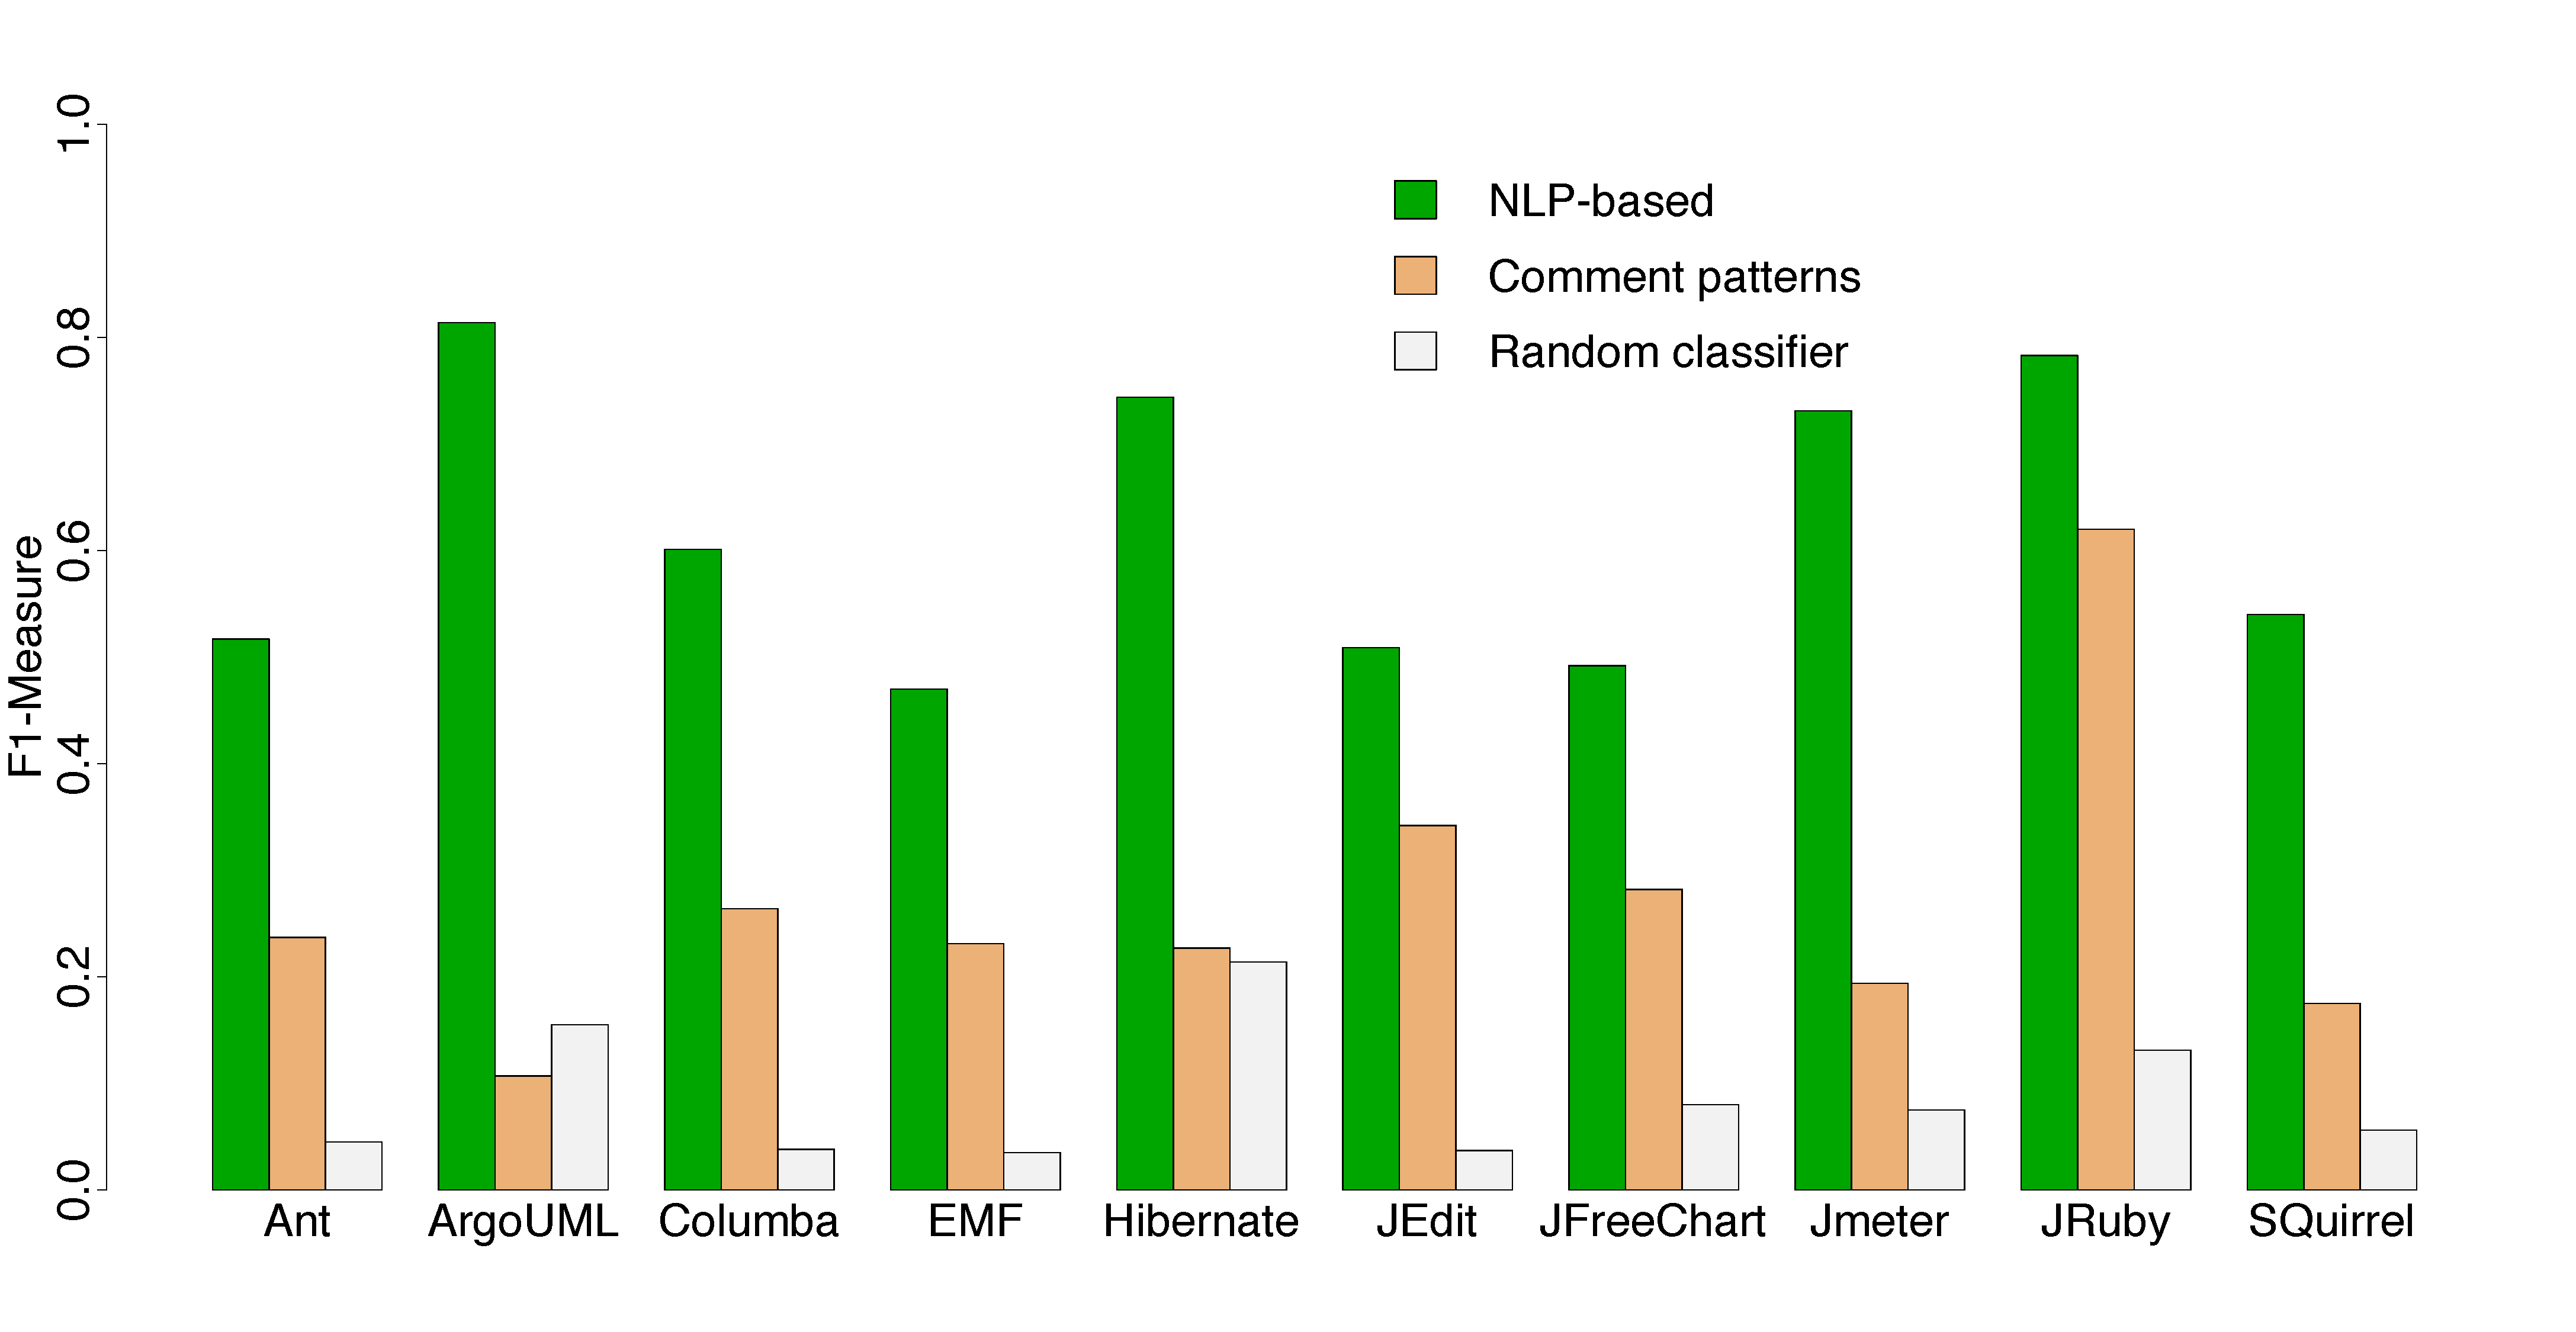
\includegraphics[width=0.48\textwidth]{figures/f1_measure_comparisom_design_1.pdf}
  \label{fig:f1_measure_comparison_design_debt}}
  \subfigure[Requirement Debt]{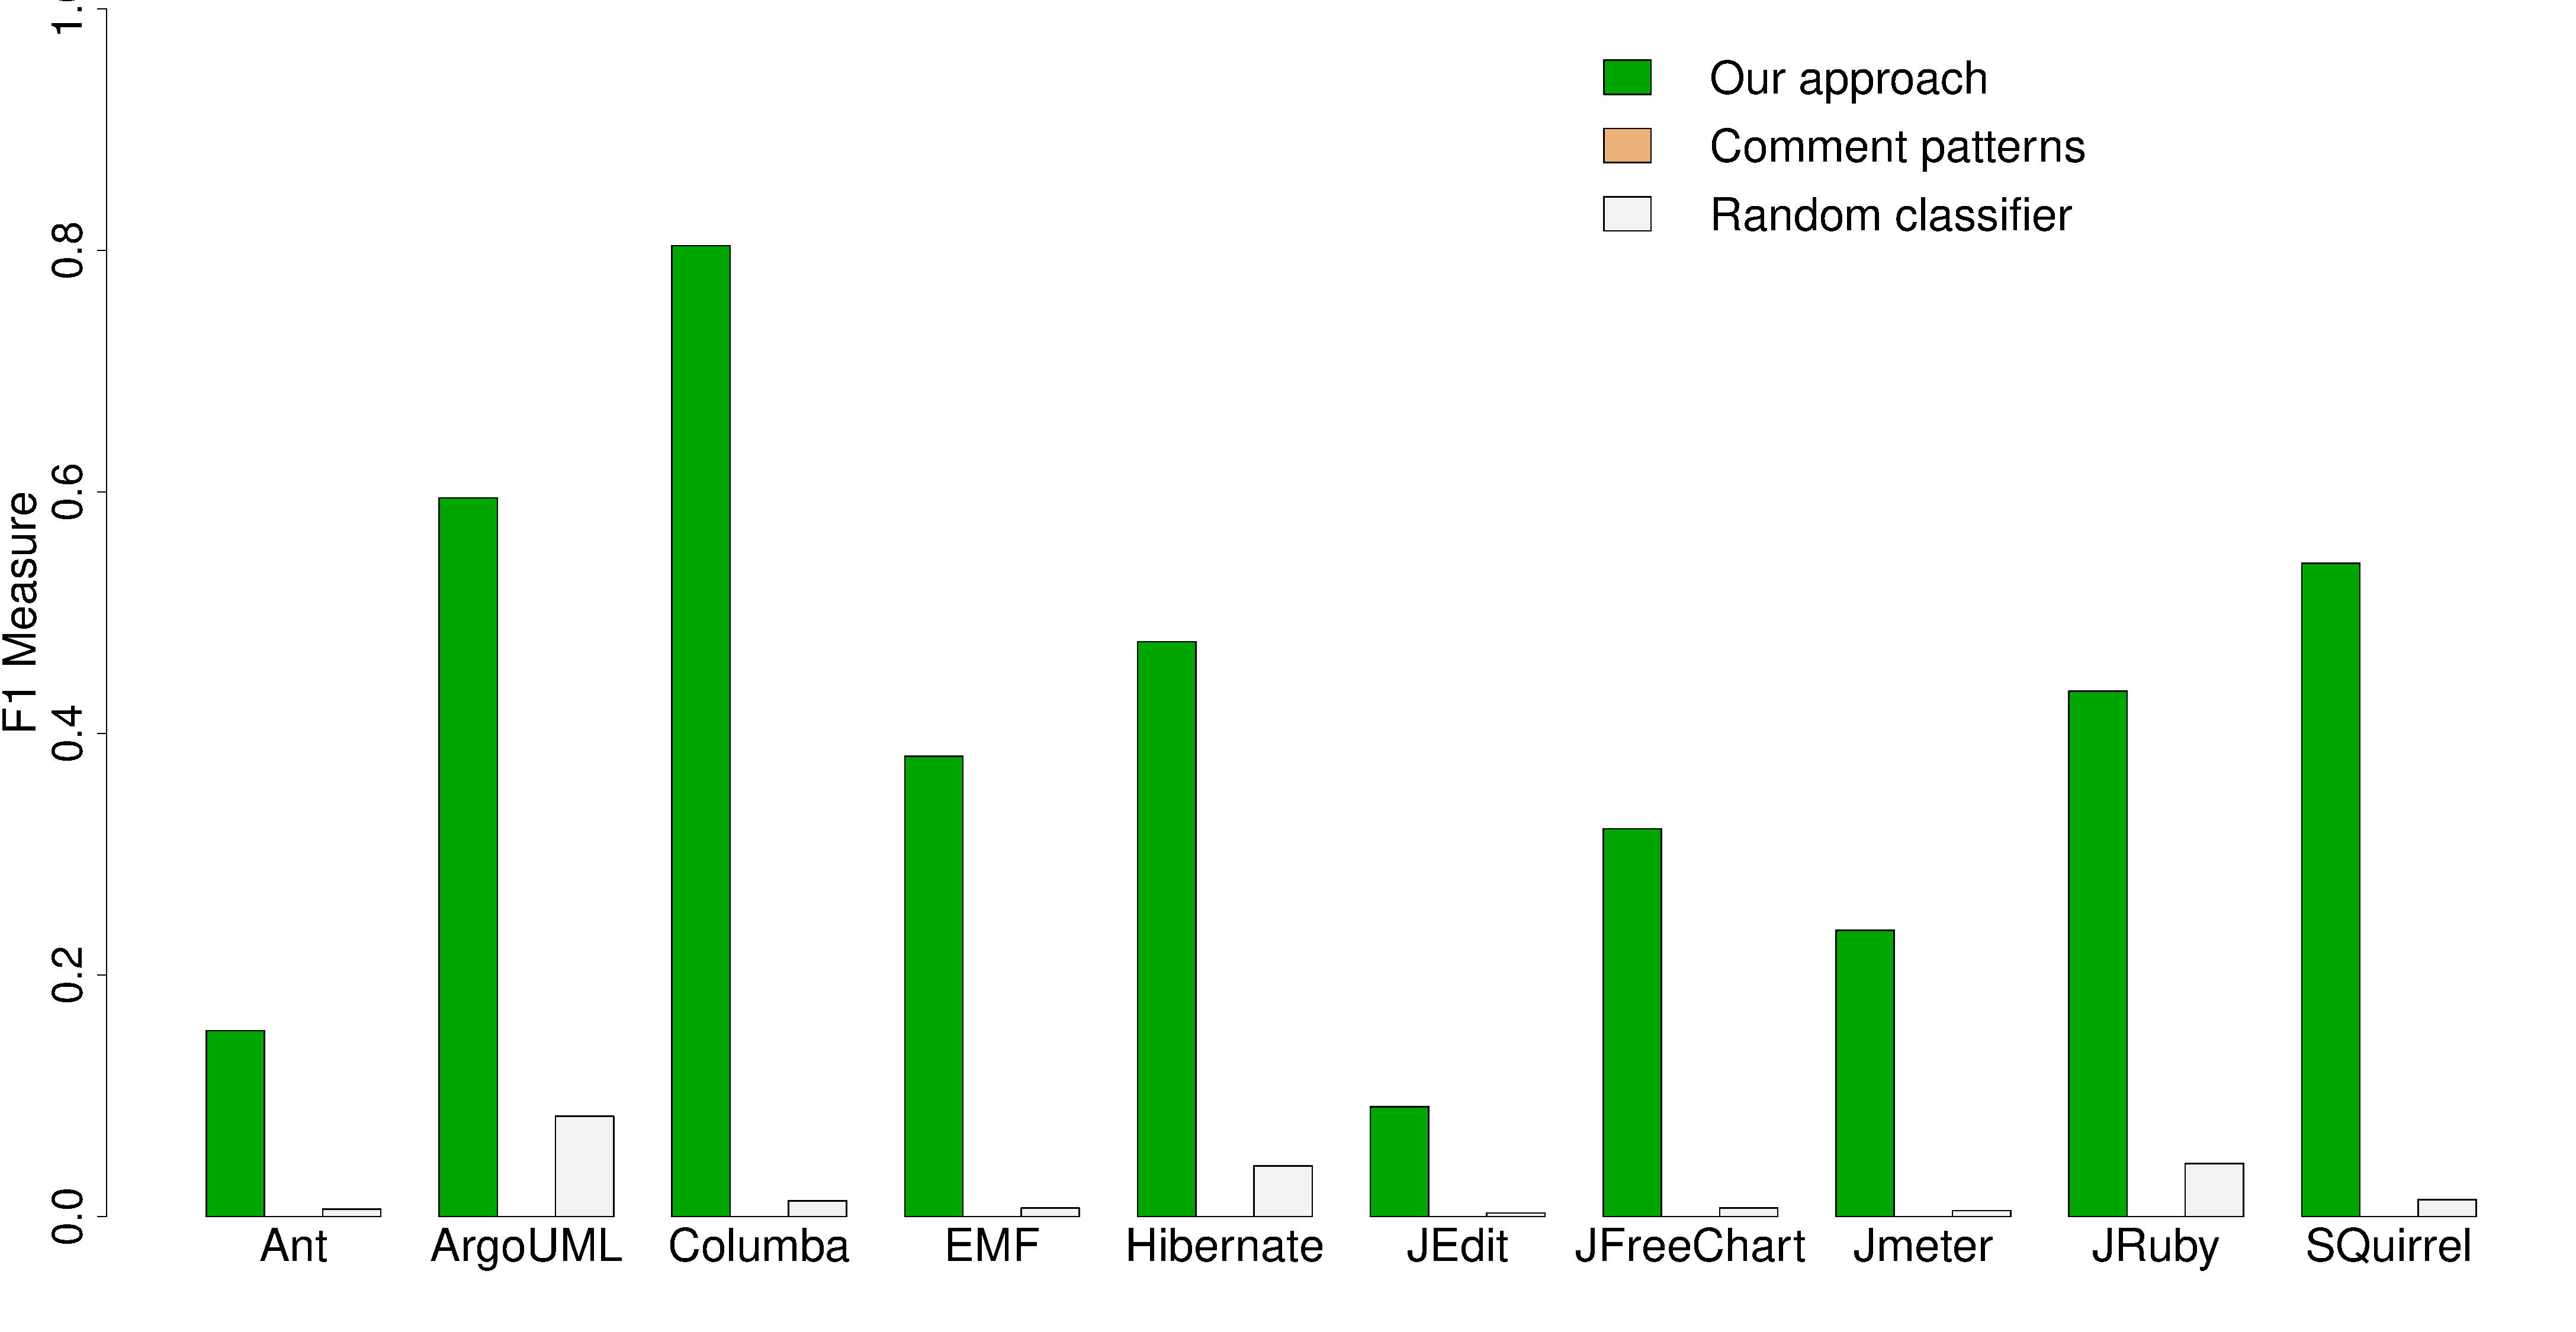
\includegraphics[width=0.48\textwidth]{figures/f1_measure_comparisom_requirement_1.pdf}
  \label{fig:f1_measure_comparison_requirement_debt}}
  \vspace{-3mm}
  \caption{Visualization of the F1-measure for Different Approaches}
\end{figure*}

\begin{table*}[!thb]
    \begin{center}
        \caption{Comparison of F1-measure Between the NLP-based, the Comment Patterns and the Random Baseline Approaches for Design and Requirement Debt}
        \label{tbl:improvement_f1measure}
        \begin{tabular}{l| c c c c c| c c c c c}
        \toprule
        
        % draw first line. The * centralizes the Project column, then set the total size of columns that we have
        \multirow{5}{*}{\textbf{\thead{Project}}} & \multicolumn{5}{c|}{\textbf{\thead{Design debt}}} & \multicolumn{5}{c}{\textbf{\thead{Requirement debt}}} 
        % indicates that from now on we are filling the content of the next line
        \\ 
        \cmidrule{2-6}
        \cmidrule{7-11}
        % remainder columns
        & {\textbf{\thead{Our\\approach}}} & {\textbf{\thead{Comment\\patterns}}} & {\textbf{\thead{Random\\classifier}}} & {\textbf{\thead{IMP over\\comment\\patterns}}} & {\textbf{\thead{IMP over\\random\\classifier}}} & {\textbf{\thead{Our\\approach}}} & {\textbf{\thead{Comment\\patterns}}} & {\textbf{\thead{Random\\classifier}}} & {\textbf{\thead{IMP over\\comment\\patterns}}} & {\textbf{\thead{IMP over\\random\\classifier}}} \\
  
        \midrule                                                  
        \textbf{Ant}       &0.517&0.237&0.045&2.1$\times$& 11.4 $\times$&0.154&0.000&0.006&-             & 25.6$\times$  \\
        \textbf{ArgoUML}   &0.814&0.107&0.155&7.6$\times$& 5.2  $\times$&0.595&0.000&0.083&-             & 7.1 $\times$  \\
        \textbf{Columba}   &0.601&0.264&0.038&2.2$\times$& 15.8 $\times$&0.804&0.117&0.013&6.8  $\times$ & 61.8$\times$  \\
        \textbf{EMF}       &0.470&0.231&0.035&2.0$\times$& 13.4 $\times$&0.381&0.000&0.007&-             & 54.4$\times$  \\
        \textbf{Hibernate} &0.744&0.227&0.214&3.2$\times$& 3.4  $\times$&0.476&0.000&0.042&-             & 11.3$\times$  \\
        \textbf{JEdit}     &0.509&0.342&0.037&1.4$\times$& 13.7 $\times$&0.091&0.000&0.003&-             & 30.3$\times$  \\
        \textbf{JFreeChart}&0.492&0.282& 0.08&1.7$\times$& 6.1  $\times$&0.321&0.000&0.007&-             & 45.8$\times$  \\
        \textbf{Jmeter}    &0.731&0.194&0.075&3.7$\times$& 9.7  $\times$&0.237&0.148&0.005&1.6 $\times$  & 47.4$\times$  \\
        \textbf{JRuby}     &0.783&0.620&0.131&1.2$\times$& 5.9  $\times$&0.435&0.409&0.044&1.0 $\times$  & 9.8 $\times$  \\
        \textbf{SQuirrel}  &0.540&0.175&0.056&3.0$\times$& 9.6  $\times$&0.541&0.000&0.014&-             & 38.6$\times$  \\
        \midrule 
        \textbf{Average}   &0.620&0.267&0.086&2.3$\times$&7.1   $\times$&0.403&0.067&0.022&6.0 $\times$  &  18 $\times$  \\ 
        \bottomrule
        \end{tabular}
    \end{center}    
\end{table*}

\vspace{3mm}
\noindent\rqi
\vspace{3mm}

\noindent \textbf{Motivation:} As shown in previous work \revised{[citation removed]}{R2-1}\cite{Maldonado2015MTD}, \SATD comments can be found in the source code. However, there is no automatic way to identify these technical debt comments. The methods proposed so far heavily rely on manual examination of source code, and there is no evidence on how well these approaches perform. Moreover, the state-of-the-art approaches to detect \SATD do not discriminate between the different types of technical debt (e.g., design, test, requirements).

Therefore, we want to determine if NLP tools such as, the \revised{maximum entropy classifier}{R2-11}, can help us surpass these limitations \revised{and outperform the detection power of the state-of-the-art approach}{R1-7}. The \revised{maximum entropy classifier}{R2-11} can automatically classify comments based on specific linguistic characteristics of these comments. Answering this question is important, since it helps us understand the opportunities and limitations of using NLP techniques to automatically identify \SATD comments. 

\vspace{1mm}
\noindent \textbf{Approach:} In this RQ, we would like to examine how effectively we can identify design and requirement \SATD. Therefore, the first step is to create a dataset that we can train and test our \revised{maximum entropy classifier}{R2-11} on. We classified the source code comments into the following types of \SATD: design debt, defect debt, documentation debt, requirement debt and test debt. However, our previous work showed that the most frequent \SATD comments are design and requirement debt. Therefore, in this paper, we focus our attention on the identification of these two types of \SATD. We decided to focus on these two types of \SATD since 1) they are the most common types of technical debt and 2) NLP-based techniques require sufficient data for training (i.e., they cannot build an accurate model with a small number of samples).

We train the \revised{maximum entropy classifier}{R2-11} using our manually created dataset. The dataset contains comments with and without \SATD, and each comment contains its own classification (i.e., without technical debt, design debt or requirement debt). Then, we add to the training dataset all comments classified as without technical debt and the comments classified as the specific type of \SATD that we want to identify. We use comments from 9 out of 10 projects that we analyzed to create the training dataset. The comments from the remaining one project are used to evaluate the classification performed by the \revised{maximum entropy classifier}{R2-11}. We choose to create the training dataset using comments from 9 out of 10 projects since we want to train the \revised{maximum entropy classifier}{R2-11} with the most diverse data possible (i.e., comments from different domains of applications). However, we discuss the implications of using training datasets of different sizes in RQ3. We repeat this process for each of the ten projects, each time training on 9 projects and testing on the remaining 1 project.

Based on the training dataset, the \revised{maximum entropy classifier}{R2-11} will classify each comment in the test dataset. The resulting classification is compared with the manual classification provided in the test dataset and evaluated. If a comment in the test dataset has the same classification as the classification suggested by the \revised{maximum entropy classifier}{R2-11}, we will have a true positive (tp) or a true negative (tn). True positives are cases where the \revised{maximum entropy classifier}{R2-11} correctly identifies \SATD comments, and true negatives are comments without technical debt that are classified as being as such. Similarly, when the classification provided by the tool diverges from the manual classification provided in the test dataset, we have false positives or false negatives. False positives (fp) are comments classified as being \SATD when they are not, and false negatives (fn) are comments classified as without technical debt when they really are \SATD comments. Using the tp, tn, fp, and fn, we are able to evaluate the performance of different detection approaches in terms of precision (i.e., $\frac{tp}{tp + fp}$), recall (i.e., $\frac{tp}{tp + fn}$) and F1-measure (i.e., $2 \times \frac{P \times R}{P + R}$). To determine how effective the NLP classification is, we compare its F1-measure with the F1-measure of two other approaches. We use the F1-measure to compare the performance between the approaches as this measurement provides the harmonic mean of precision and recall. Using the F1-measure allows us to incorporate the tradeoff between precision and recall and present one value that evaluates both measures.

The first approach is the current state-of-the-art in detecting \SATD comments \revised{[citation removed]}{R2-1}. This approach uses 62 comment patterns (i.e., keywords and phrases) that were noticed as recurrent in \SATD comments during the manual inspection of 101,762 comments. The second approach is a simple (random) baseline, which assumes that the detection of \SATD is random (this approach is used as a performance lower bound). The precision of this approach is calculated by taking the total number of \SATD over the total number of comments of each project. For example, Ant has 4,137 comments, of those, only 95 comments are design \SATD. The chance of randomly finding a design \SATD comment is 0.022 (i.e., $\frac{95}{4,137}$). Similarly, to calculate the recall we take into consideration the two possible classifications available: one is the type of \SATD (e.g., design) and the other is without technical debt. Therefore, there is a 50\% chance that the comment will be a \SATD. 

\vspace{1mm}

\noindent \textbf{Results - design debt:} Table \ref{tbl:improvement_f1measure} presents the F1-measure of the three approaches, as well as the improvement achieved by our approach compared to the other two approaches. We see that for all the projects, the F1-measure achieved by our approach is higher than the other approaches F1-measures. The F1-measure obtained by our NLP-based approach ranges between 0.470 - 0.814, with an average of 0.620. In comparison, the F1-measure using the comment patterns ranges between 0.107 - 0.620, with an average of 0.267, and the simple (random) baseline approach achieves F1-measures in the range of 0.035 - 0.214, with an average of 0.086. Figure \ref{fig:f1_measure_comparison_design_debt} visualizes the comparison of the F1-measure for our NLP-based approach, the comment patterns approach and the simple (random) baseline approach. We see from both, Table \ref{tbl:improvement_f1measure} and Figure \ref{fig:f1_measure_comparison_design_debt} that, on average, our approach outperforms the state-of-the-art comment pattern approach by 2.3 times and the simple (random) baseline approach by a factor of 7.1 times when identifying design \SATD.

It is important to note that the comment patterns approach has a high precision, but it lacks recall, i.e., this approach points correctly to \SATD comments, but as the approach depends on keywords, it identifies a very small subset of all the \SATD comments in the project. Although we only present the F1-measures in here, we present the precision and recall values in Table~\ref{tbl:classifier_results_vs_baseline_design} located in the Appendix section.  

\noindent \textbf{Results - requirement debt:} \revised{Similarly, the last five columns of Table \ref{tbl:improvement_f1measure} presents the F1-measure performance of the three approaches, and the improvement achieved by our approach over the two other approaches. The comment patterns approach was able to identify requirement \SATD in 3 of the 10 analyzed projects. A possible reason for the low performance of the comment patterns in detecting requirement debt is that the authors of the comment patterns approach did not differentiate between the different types of \SATD when deriving their patterns. Moreover, since most of the debt is design debt, it is possible that the patterns tend to favor the detection of design debt.}{R1-9} 
 
That said, we find that for all projects, the F1-measure obtained by our approach surpasses the other approaches F1-measures. Our approach achieves a F1-measure between 0.091 - 0.804 with an average of 0.403, whereas the comment pattern approach achieves F1-measure in the range of 0.117 - 0.409 with an average of 0.067. In comparison, the simple (random) baseline ranges between 0.003 - 0.083, with an average of 0.022. Figure \ref{fig:f1_measure_comparison_requirement_debt} visualizes the performance comparison of the two approaches.\revised{We also test the F1-measure obtained by our approach with the other two baselines to determine if the differences in value are statistically significant. We find that the differences are indeed statistically significant (i.e., p\textless0.5) for the comment patterns and the random classifier baselines for both design and requirement \SATD.}{R3-6}

Generally, it is clear that requirement \SATD is less common than design \SATD, which makes it more difficult to detect.\revised{ Nevertheless, our NLP-based approach provides a significant improvement over the comment patterns approach and the simple (random) baseline approach, with an average improvement of 7 and 18 times, respectively.}{R1-9} The tables in this section only present the F1-measure values for brevity reasons, however, we present the detailed precision and recall values in the Appendix section, Table \ref{tbl:classifier_results_vs_baseline_requirement}.

\revised{\conclusionbox{We find that our NLP-based approach, is more effective in identifying self-admitted technical debt comments compared to the the current state-of-art approaches. We achieved an average F1-measure of 0.620 when identifying design debt (an average improvement of 2.3x over the state-of-the-art approach) and an average F1-measure of 0.403 when identifying requirement debt (an average improvement of 6x over the state-of-the-art approach).}}{R1-8}

\vspace{3mm}
\noindent\rqii
\vspace{3mm}

\noindent \textbf{Motivation:} After asserting the efficiency of our NLP-based approach in identifying \SATD comments we want to better understand what words developers use when indicating this technical debt. Answering this question will provide insightful information that can guide future research directions, broaden our understanding on \SATD and also help us to detect it.     

\vspace{1mm}
\noindent \textbf{Approach:} To perform its detection, the \revised{maximum entropy classifier}{R2-11} learns optimal features that can be used to detect \SATD. These features, are fragments of data (e.g., words) that are associated with a specific class (i.e., design debt, requirement debt, or without technical debt). Moreover, each feature has a weight, which represents how strongly the feature relates to a specific type of debt. The \revised{maximum entropy classifier}{R2-11} uses the classified training data that we input to determine the features and their weigh. Then, the features and their corresponding weights are used to determine if a comment belongs to a specific type of \SATD.

For example, if the \revised{maximum entropy classifier}{R2-11}, based on the training data, determines that the two features ``hack'' and ``dirty'' are related to design debt with weight 5.3 and 3.2, respectively, and the feature ``something'' relates to the without technical debt class with a weight of 4.1. Then, if we aim to classify the comment ``this is a dirty hack it's better to do something'' in our test data, all features will be analyzed and the following score would be calculated: design debt weight = 8.5 (i.e., feature `hack' weight plus feature `dirty' weight) and without technical debt weight = 4.1 resulting in a comment classified as design debt.

For each analyzed project, we collect the features used to identify the \SATD comments. These features are provided by the \revised{maximum entropy classifier}{R2-11} as output and stored in a text file. The features are written in the file based on the weight that they have, ordered by highest weight to the lowest weight, meaning more relevant features to less relevant features respectively. Based on these files, we rank the words calculating the average ranking position of the analyzed feature across the ten different projects. 

\noindent \textbf{Results:} Table \ref{tbl:top_ten_features} shows the top 10 textual features used to identify  \SATD in the ten studied projects, ordered by their relevance. The first column we present the ranking of each textual feature, the second column lists the features used in the identification of \emph{design} \SATD, and the third column lists the textual features used to identify \emph{requirement} \SATD.

\begin{table}[!thb]
    \begin{center}
        \caption{Top Ten Textual Features Used to Identify Design and Requirement Self-Admitted Technical Debt}
        \label{tbl:top_ten_features}
        \begin{tabular}{l| l l }
        \toprule
        \textbf{Rank} & \textbf{Design Debt} & \textbf{Requirement Debt}  \\
        \midrule
         \textbf{1}  & hack       &   todo              \\
         \textbf{2}  & workaround &   needed            \\
         \textbf{3}  & yuck!      &   implementation    \\
         \textbf{4}  & kludge     &   fixme             \\
         \textbf{5}  & stupidity  &   xxx               \\
         \textbf{6}  & needed?    &   ends?             \\
         \textbf{7}  & columns?   &   convention        \\
         \textbf{8}  & unused?    &   configurable      \\
         \textbf{9}  & wtf?       &   apparently        \\
         \textbf{10} & todo       &   fudging           \\
        \bottomrule
        \end{tabular}
    \end{center}    
\end{table}

From Table~\ref{tbl:top_ten_features} we observe that the top ranked textual features, i.e., hack, workaround, yuck!, kludge and stupidity, are related to design \SATD indicate sloppy or mediocre source code. For example we have the following comment that was extracted from Jmeter: \textit{``\textbf{Hack} to allow entire URL to be provided in host field''}. Other textual features such as needed?, columns?, unused?, wtf? and todo, are questioning the usefulness or utility of specific source code. As this other comment, also extracted from Jmeter, shows: \textit{``TODO: - is this \textbf{needed?}''}.\revised{For requirement \SATD, the top ranked features, i.e., todo, needed, implementation, and fixme, indicate the need to complete requirements in the future that are currently partially completed. This comment from JRuby is an example: \textit{``\textbf{TODO:} implement, won't do this now''}. Other lower ranked textual features such as xxx, ends?, convention, configurable, apparently and fudging, indicate potential incomplete requirements that would make the code more configurable and/or generic.}{R1-11}

We also observe that it is possible for a single textual feature to indicate both design and requirement \SATD. However, in such cases, the ranking of the textual features for design and requirement \SATD is different. For example, the word ``todo'' is ranked tenth for design debt, whereas it is ranked first for requirement debt. This finding is intuitive, since requirement debt will naturally be related to the implementation of future functionality.

It is important to note here that although we present the top 10 textual features, the classification of the comments can be based on a combination of several textual features. In fact, two different types of textual features are used to classify the comments: positive weight features and negative weight features. Positive weight features will increase the total weight of the vote suggesting that the classification should be equal to the class of the feature (i.e., design or requirement debt). On the other hand, negative weight features will decrease the total weight of the vote suggesting a classification different from the class that the feature belongs (i.e, without technical debt). On average, the number of positive weight features used to classify design debt is 5,014 and 2,195 for requirement debt. The exact number of unique textual features used to detect \SATD for each project is shown in Table \ref{tbl:features_per_project}. The fact that our NLP-based approach leverages so many features helps to explain the significant improvement we are able to achieve over the state-of-the-art \revised{[citation removed]}{R2-1}, which only uses 62 patterns. In comparison, our approach leverages 35,828 unique textual features for design debt and 34,056 unique textual features to detect requirement debt.

\begin{table*}[!hbt]
    \begin{center}
        \caption{Number of Unique Textual Features Use to Detect Design and Requirement Debt for Each Project}
        \label{tbl:features_per_project}
        \begin{tabular}{l| c c c|| c c c}
        \toprule
        \multirow{4}{*}{\textbf{\thead{Project}}} & \multicolumn{3}{c||}{\textbf{\thead{Design debt}}} & \multicolumn{3}{c}{\textbf{\thead{Requirement debt}}} 
        \\
        \cmidrule{2-7}
        & \textbf{\thead{Positive\\Weight\\Features}} & \textbf{\thead{Negative\\Weight\\Features}} & \textbf{\thead{\# of\\Features}} & \textbf{\thead{Positive\\Weight\\Features}} & \textbf{\thead{Negative\\Weight\\Features}} & \textbf{\thead{\# of\\Features}}\\
        \midrule
        \textbf{Ant}          & 5,299 & 23,623 & 28,922 & 1,812 & 27,673 & 29,485 \\
        \textbf{ArgoUML}      & 3,917 & 26,012 & 29,929 & 2,779 & 27,260 & 30,039 \\
        \textbf{Columba}      & 5,255 & 24,182 & 29,437 & 2,433 & 27,561 & 29,994 \\
        \textbf{EMF}          & 5,346 & 23,667 & 29,013 & 1,889 & 27,637 & 29,526 \\
        \textbf{Hibernate}    & 4,914 & 24,070 & 28,984 & 2,748 & 26,654 & 29,402 \\
        \textbf{JEdit}        & 5,042 & 24,644 & 29,686 & 1,831 & 28,267 & 30,098 \\
        \textbf{JFreeChart}   & 5,361 & 23,530 & 28,891 & 1,902 & 27,439 & 29,341 \\
        \textbf{Jmeter}       & 5,172 & 23,916 & 29,088 & 1,893 & 27,716 & 29,609 \\
        \textbf{JRuby}        & 4,856 & 24,553 & 29,409 & 2,850 & 27,085 & 29,935 \\
        \textbf{SQuirrel}     & 4,982 & 25,146 & 30,128 & 1,814 & 26,914 & 28,728 \\
        \midrule
        \textbf{Average}       & 5,014 & 24,334 & 29,348 & 2,195  & 27,420 & 29,615 \\      
        \textbf{Total unique}  & 6,327  & 31,518 & 35,828   & 4,015  & 32,954 & 34,056 \\
        \bottomrule
        \end{tabular}
    \end{center}    
\end{table*}

\begin{figure*}[!thb]
	\centering
	\subfigure[Ant Design Debt Classification]{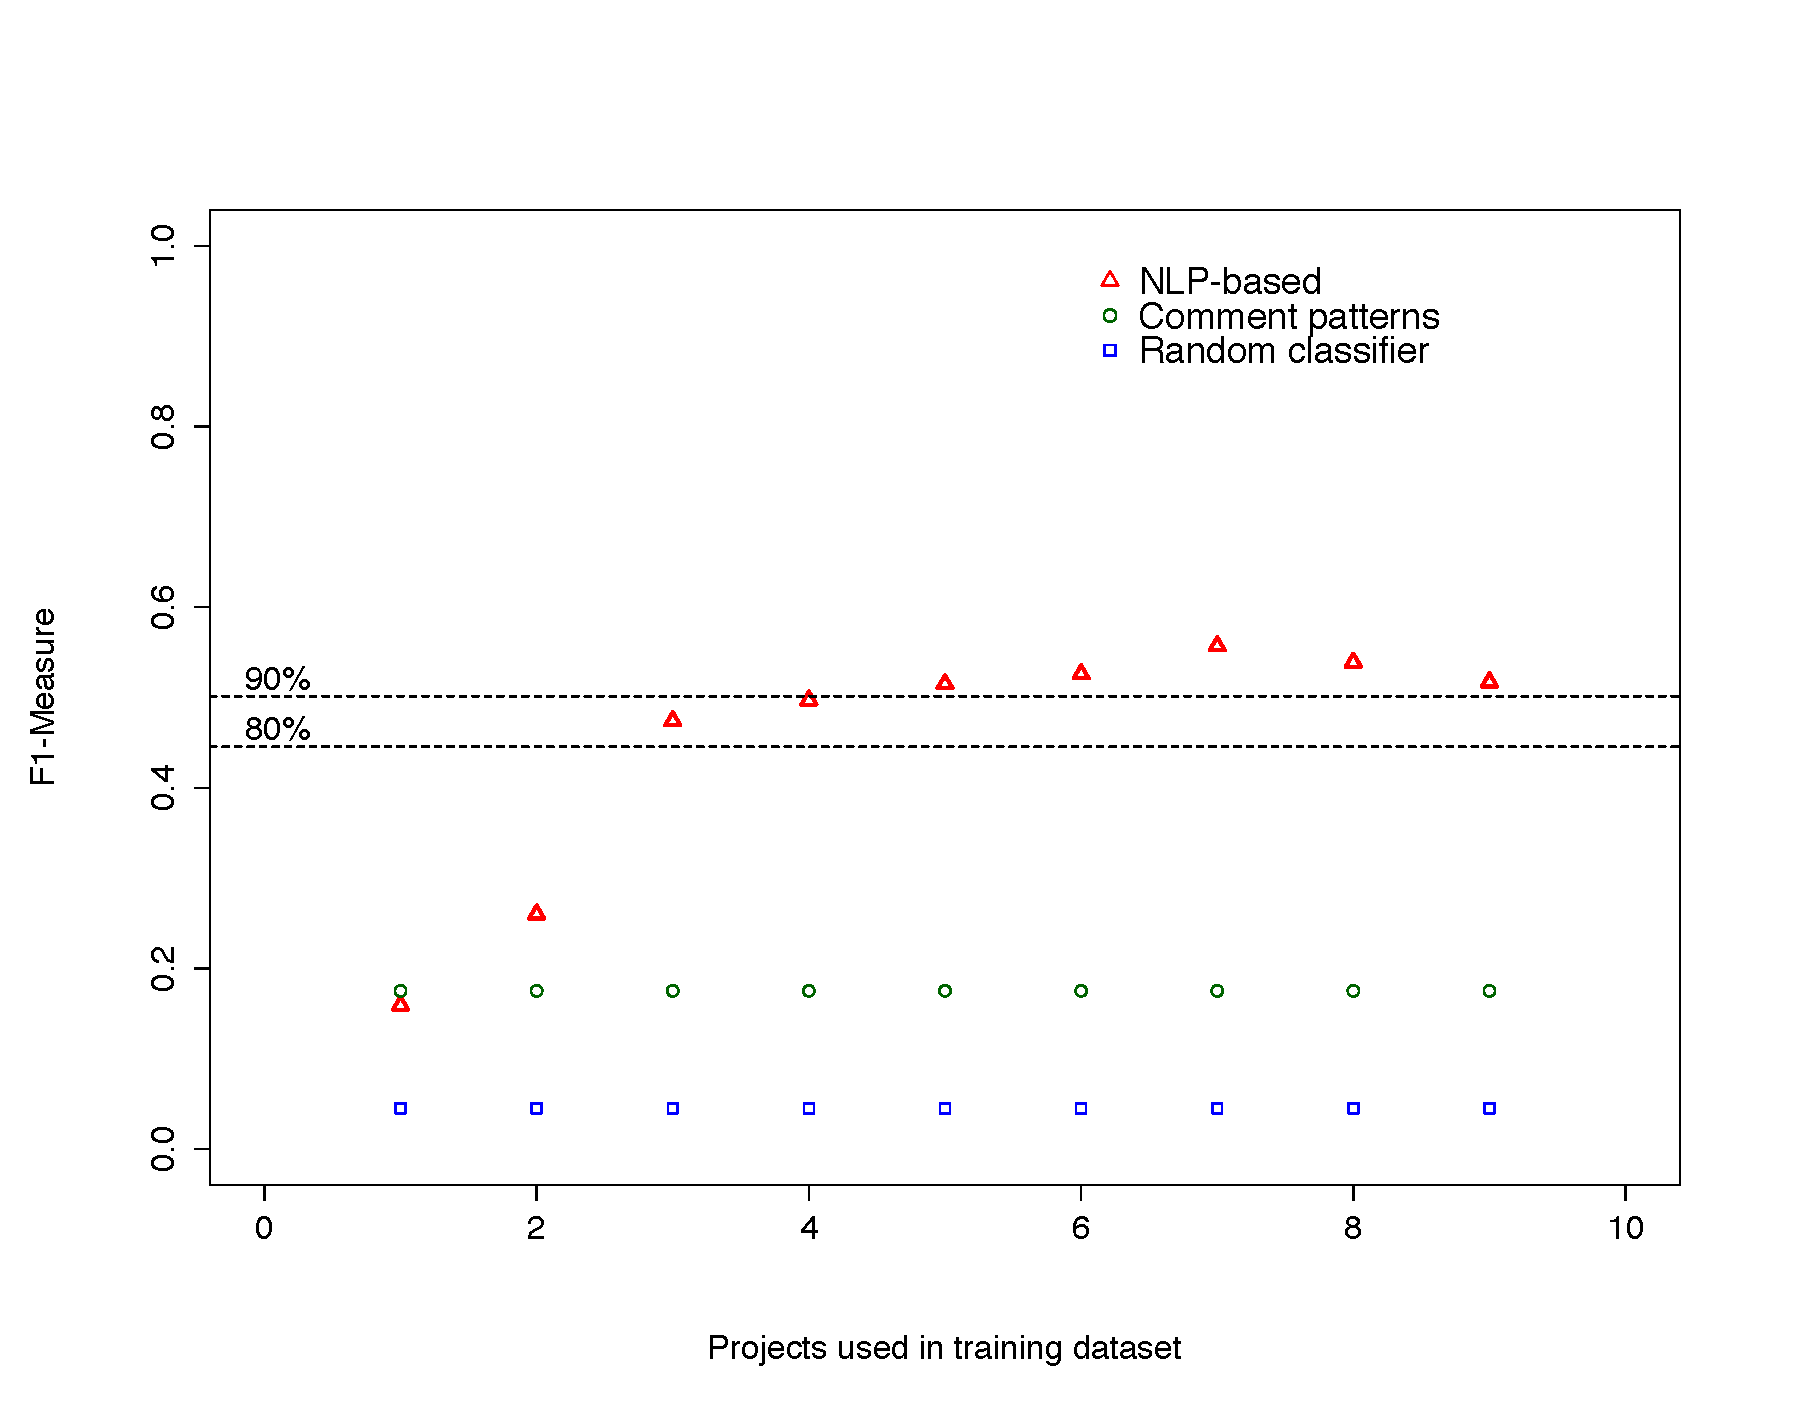
\includegraphics[width=0.49\textwidth]{figures/design_ant.pdf}
		\label{fig:design_ant_result}}
        \subfigure[Design Debt Average Percentage of F1-measure]{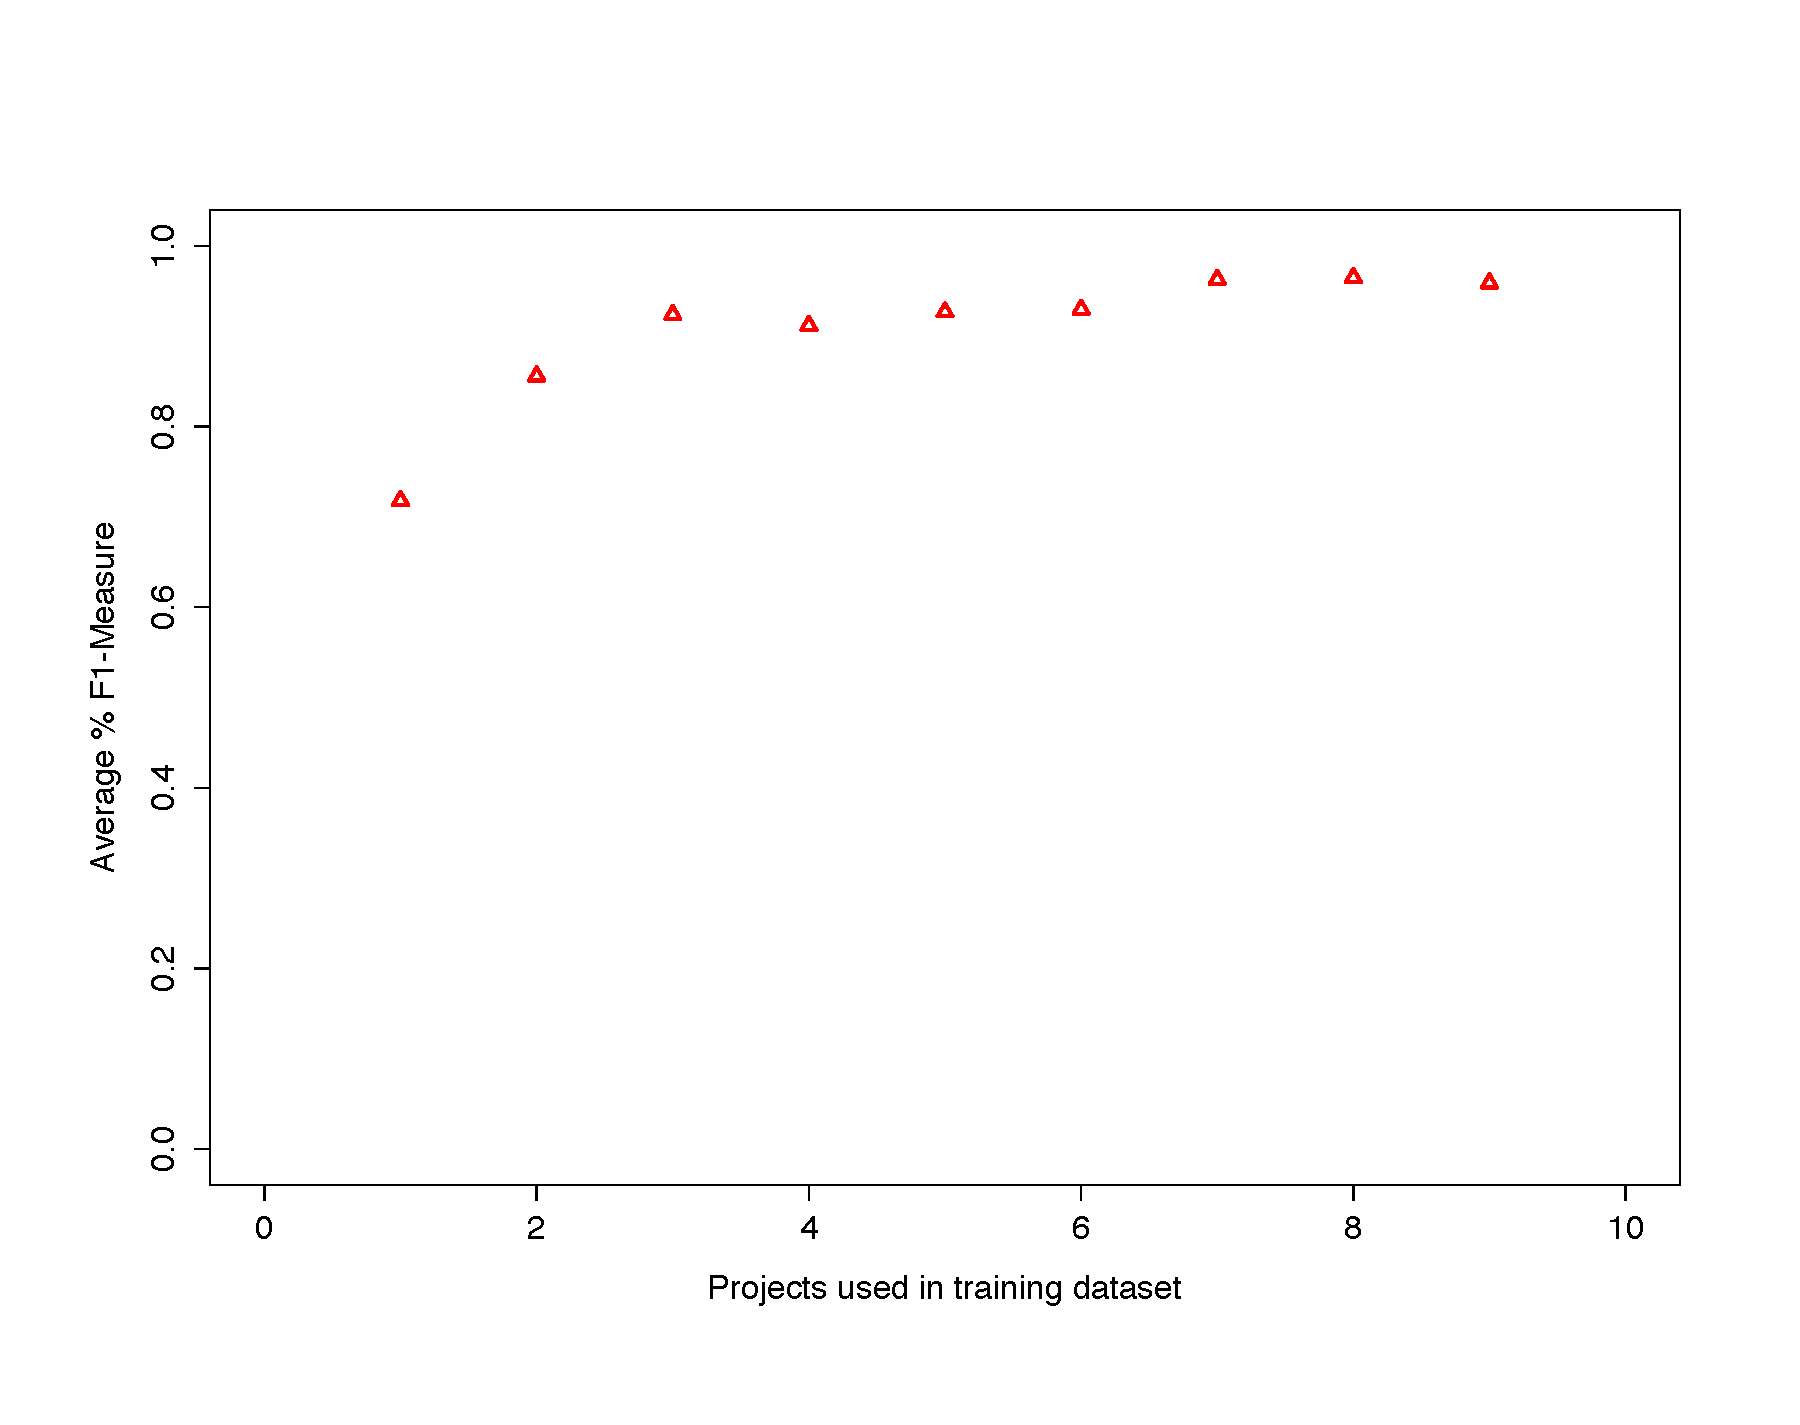
\includegraphics[width=0.49\textwidth]{figures/design_percentage_f1_measure.pdf}
    \label{fig:design_percentage_f1_measure}}

    
	\subfigure[ArgoUml Requirement Debt Classification]{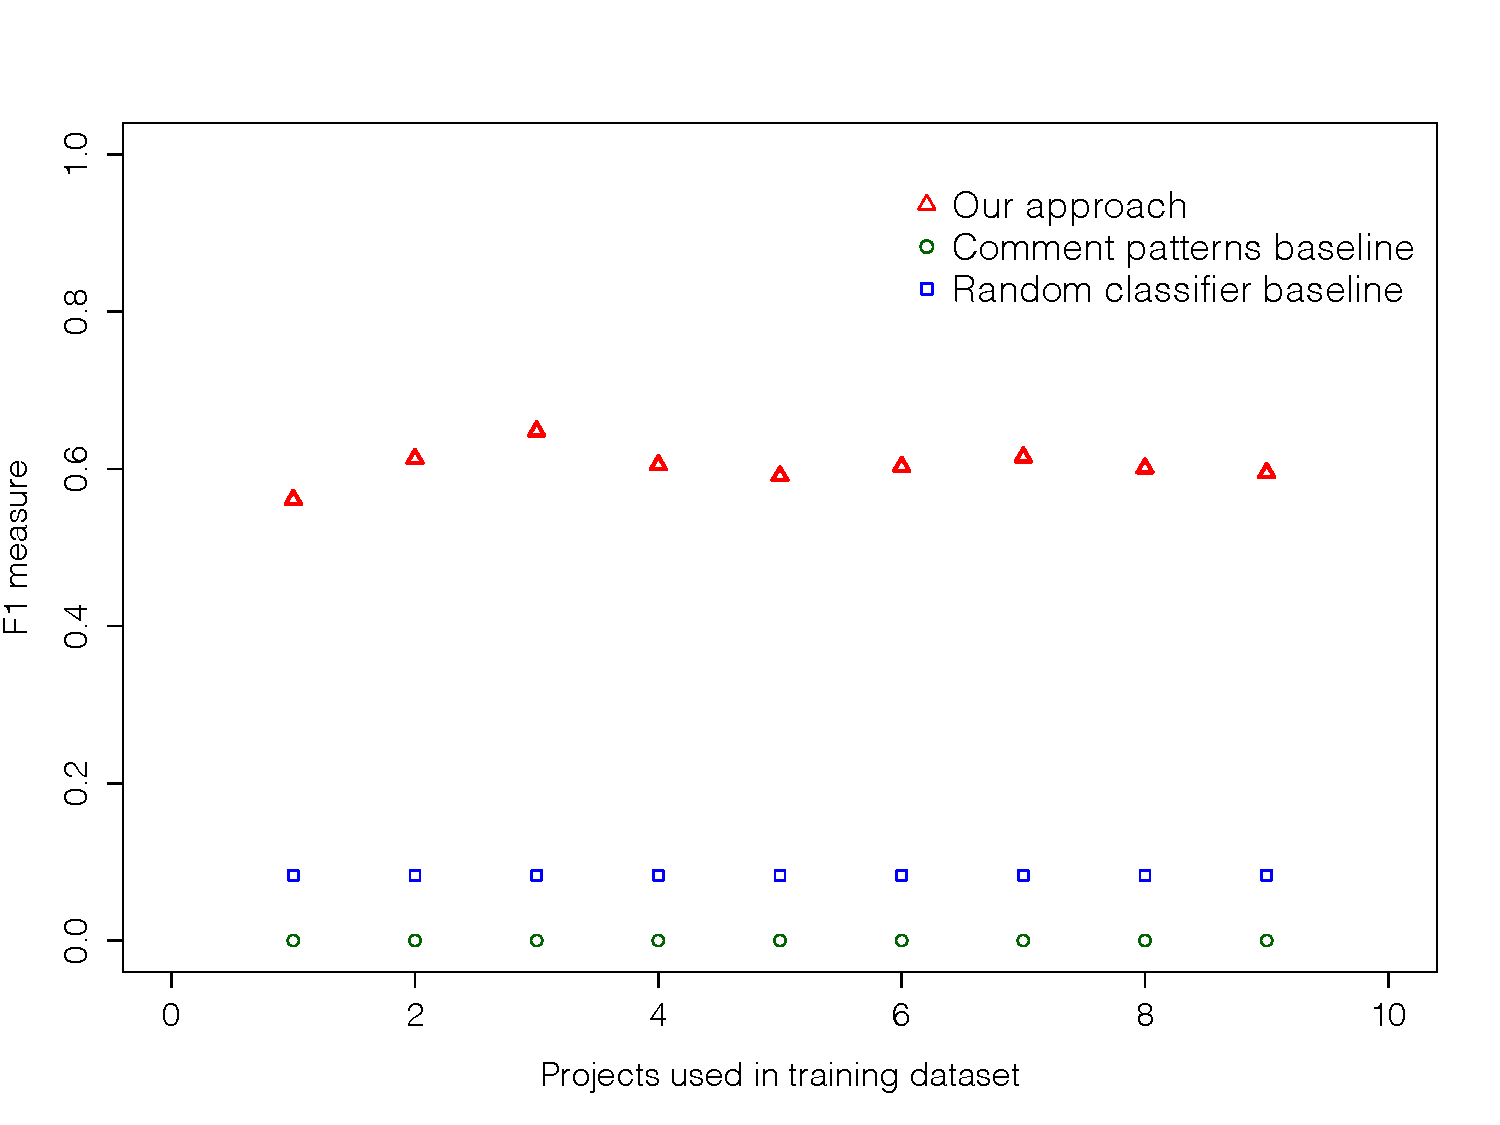
\includegraphics[width=0.49\textwidth]{figures/implementation_argo.pdf}
		\label{fig:implementation_argo_result}}
        \subfigure[Requirement Debt]{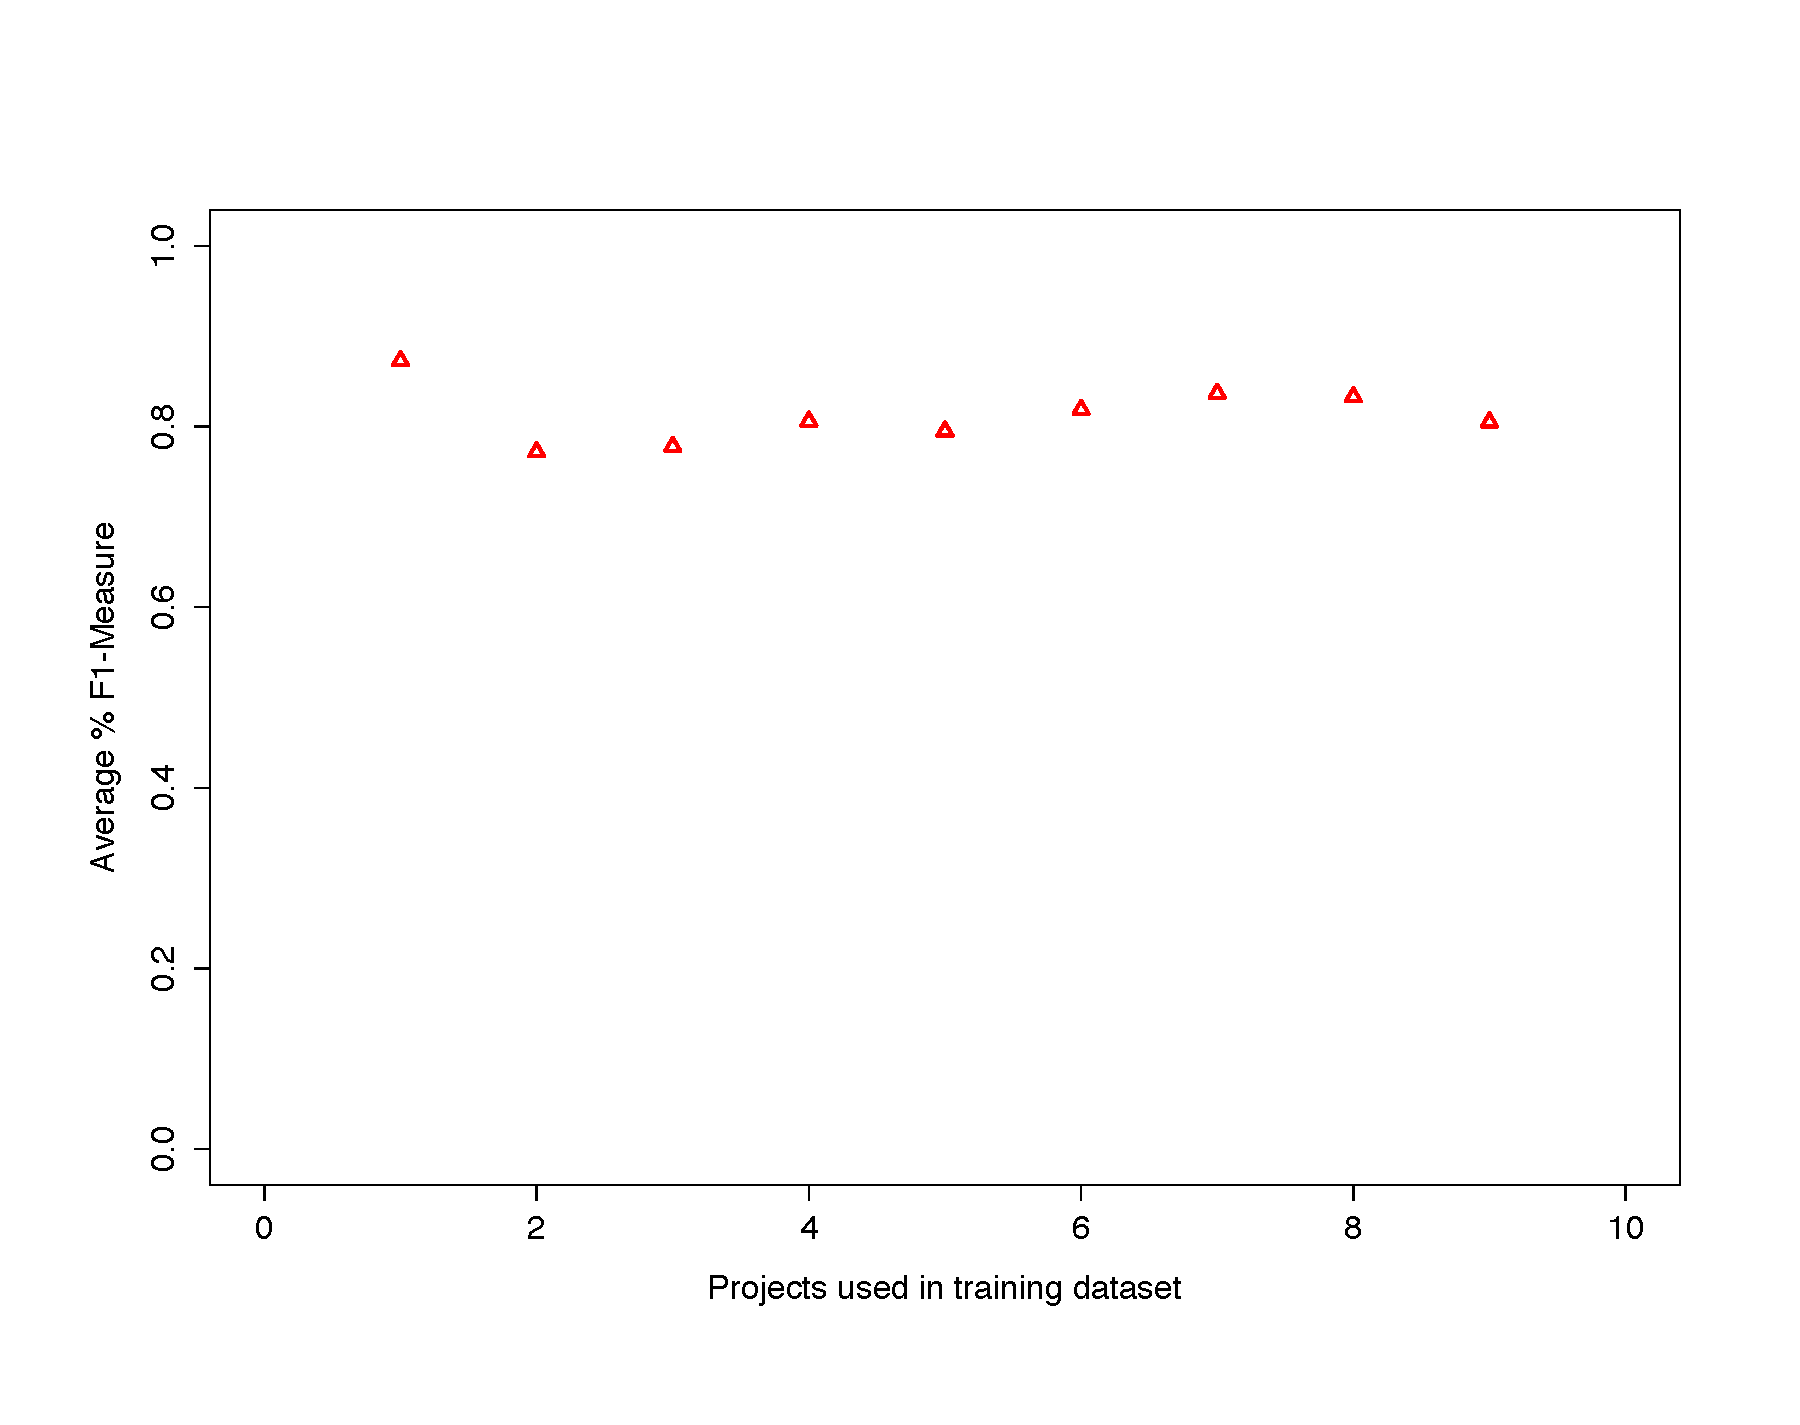
\includegraphics[width=0.49\textwidth]{figures/requirement_percentage_f1_measure.pdf}
    \label{fig:requirement_percentage_f1_measure}}
	\caption{F1-measure Achieved per Iteration }
\end{figure*}



\conclusionbox{We find the that design and requirement debt have their own textual features that best indicate such \SATD comments. For design debt, the best indicative textual features indicate sloppy or mediocre source code, whereas for requirement debt they relate to the need to enhance or complete the implementation in the future.}

\vspace{3mm}
\noindent\rqiii
\vspace{3mm}

\noindent \textbf{Motivation:} Thus far, we have shown that our NLP-based approach can effectively identify \SATD comments. However, we conjuncture that the performance of the classification depends on the amount of training data. At the same time, creating the training dataset is expensive and manually intensive. So, the question that arises is: how much training data do we need to effectively classify the \SATD comments? If we need a high number of comments to create our training dataset, our approach will be more difficult to extend and applied for other projects. On the other hand, if a small dataset can be used to identify \SATD comments, then this approach can be applied with minimal effort, i.e., less training data. That said, intuitively we expect that the performance of the \revised{maximum entropy classifier}{R2-11} would improve as more comments are being added to the training dataset.

\noindent \textbf{Approach:} To answer our research question, \revised{we conducted two different experiments. On both of them we followed a systematic process where we incrementally add training data and evaluate the performance of the classification. However, for the first experiment we added training data in a per-project basis (i.e., a variable number of comments all belonging to the same project at the same time), whereas for the second experiment, we added data 100 comments at a time regardless of the project that it belongs. 

To execute the first experiment, we use one project as testing data, and the remaining nine projects to train, since we have 10 projects in our dataset.}{R2-14} However, we do not train the \revised{maximum entropy classifier}{R2-11} with all nine projects, instead, we add each project incrementally. We repeated this process for each project and report on our findings.

\revised{It is important to notice that the order we added each project was not aleatory. After some experimentation we decided that the best way to train the max entropy classifier is to add first to the training dataset projects with more of the \SATD comments being identified. This way we could achieve better classification performance quicker. Furthermore, adding projects in a randomly fashion would impact the classification performance and prevent us to properly analyze the results of the first experiment.}{R2-15}

To determine how much data is required to effectively identify \SATD comments, we compute the F1-measure after each iteration (an iteration is simply a run with a different size of training data). We record the iteration that achieves the highest F1-measure and the number of projects used in the training dataset to achieve this F1-measure. Then, we record the number of projects needed to achieve at least 90\% and 80\% of the maximum F1-measure.

For example, if the maximum F1-measure is 0.85 and it is achieved in the eighth iteration (i.e., using 8 projects in the training dataset), and during the fourth iteration we achieve a F1-measure of 0.80, then we say that we can achieve at least 90\% (94\% to be exact) of the maximum F1-measure with a training dataset constructed from just 4 projects. Since the results will differ for the different projects, we repeat this analysis for all projects and present the average F1-measures across all projects.

\revised{To execute the second experiment, we shuffle the comments from all projects into a big dataset. Then, we split this dataset into 10 identical parts making sure that each part has an identical ratio of \SATD and without technical debt comments. Next, we use one of the ten parts to test the max entropy classifier and the other 9 to train it. The training data is incrementally feed into the classifier by batches of 100 comments at time, and we also make sure that each batch of 100 comments contains the same ratio of \SATD and without technical debt comments. We repeated this process for each one of the 10 dataset parts and report on our findings.

For this experiment, to determine how much data is required to effectively identify \SATD comments we also compute the F1-measure after each iteration and record the iteration that achieves the highest F1-measure. However, instead of recording the number of projects that were used to train the dataset we report the number of comments that was used to achieve this F1-measure. The number of comments is computed in multiples of 100, due to the size of each batch added to the training dataset.

\noindent \textbf{Per-project based experiment results - design debt:}}{R2-14} Figure~\ref{fig:design_ant_result} shows the F1-measure using different sizes of training data for the Ant project. Due to space, we discuss the results for a representative project (Ant) in this section, however, \revised{Figure~\ref{fig:design_percentage_f1_measure} presents the maximum percentage average achieved for all projects in each one of the analyzed iterations.}{R3-9}. From Figure~\ref{fig:design_ant_result}, we find that the maximum F1-measure improves as we increase the number of projects (i.e., iterations), achieving the highest F1-measure in the seventh iteration and slightly decreasing afterwards. The horizontal lines in the figure show the 80\% and 90\% of the highest F1-measure. We can see from Figure~\ref{fig:design_ant_result} that with 1,499 comments (i.e., from 3 projects) and 1,815 comments (i.e., from 4 projects), we can achieve 80\% and 90\% of the highest F1-measure, respectively. This amounts to a reduction of  37.6\% and 24.5\% in training data to achieve 80\% and 90\% of the maximum F1-measure, respectively. Considering the tradeoff in accuracy versus the amount of training data, for Ant, using only 3 or 4 projects provides the best tradeoff.

We analyzed all iterations from all projects to determine the iterations that achieve the best F1-measure performance. To measure that, we calculate the average percentage of the maximum F1-measure for each iteration\revised{as shown in Figure~\ref{fig:design_percentage_f1_measure}}{R3-9}. For example, we take the average percentage of the maximum F1-measure achieved during the first iteration for all projects, then we calculate the same value for all second iterations and so on. We find that, the best performance is achieved during the eighth iteration, with an average maximum F1-measure of 96.57\% using (on average) 2,353 comments to create the training dataset. In comparison, the ninth iteration has an average  maximum F1-measure of 95.99\%, which is slightly lower than the average obtained in the eighth iteration, and uses more comments in the training dataset (i.e., 2,432).

Table \ref{tbl:design_iteration_performance} shows the average percentage of the maximum F1-measure for each iteration. The first column shows the iteration number. The second column shows the average percentage of the maximum F1-measure achieved for each iteration. The third column presents the delta of the average percentage of the maximum F1-measure between one iteration and the previous one. The fourth column shows the average number of comments used in the training dataset of that specific iteration. From Table~\ref{tbl:design_iteration_performance} we observe that, on average, we can achieve more than 80\% and 90\% of the maximum F1-measure in the second and third iterations, respectively. To achieve more than 80\% and 90\% of the maximum F1-measure, we require 1,106 (49.13\% of total comments required in seventh iteration) and 1,444 (64.14\% of total comments required in seventh iteration) comments, respectively. Moreover, we see that the second and third iterations provide the highest delta between iterations.

\begin{figure*}[!thb]
    \centering
    \subfigure[Design Debt]{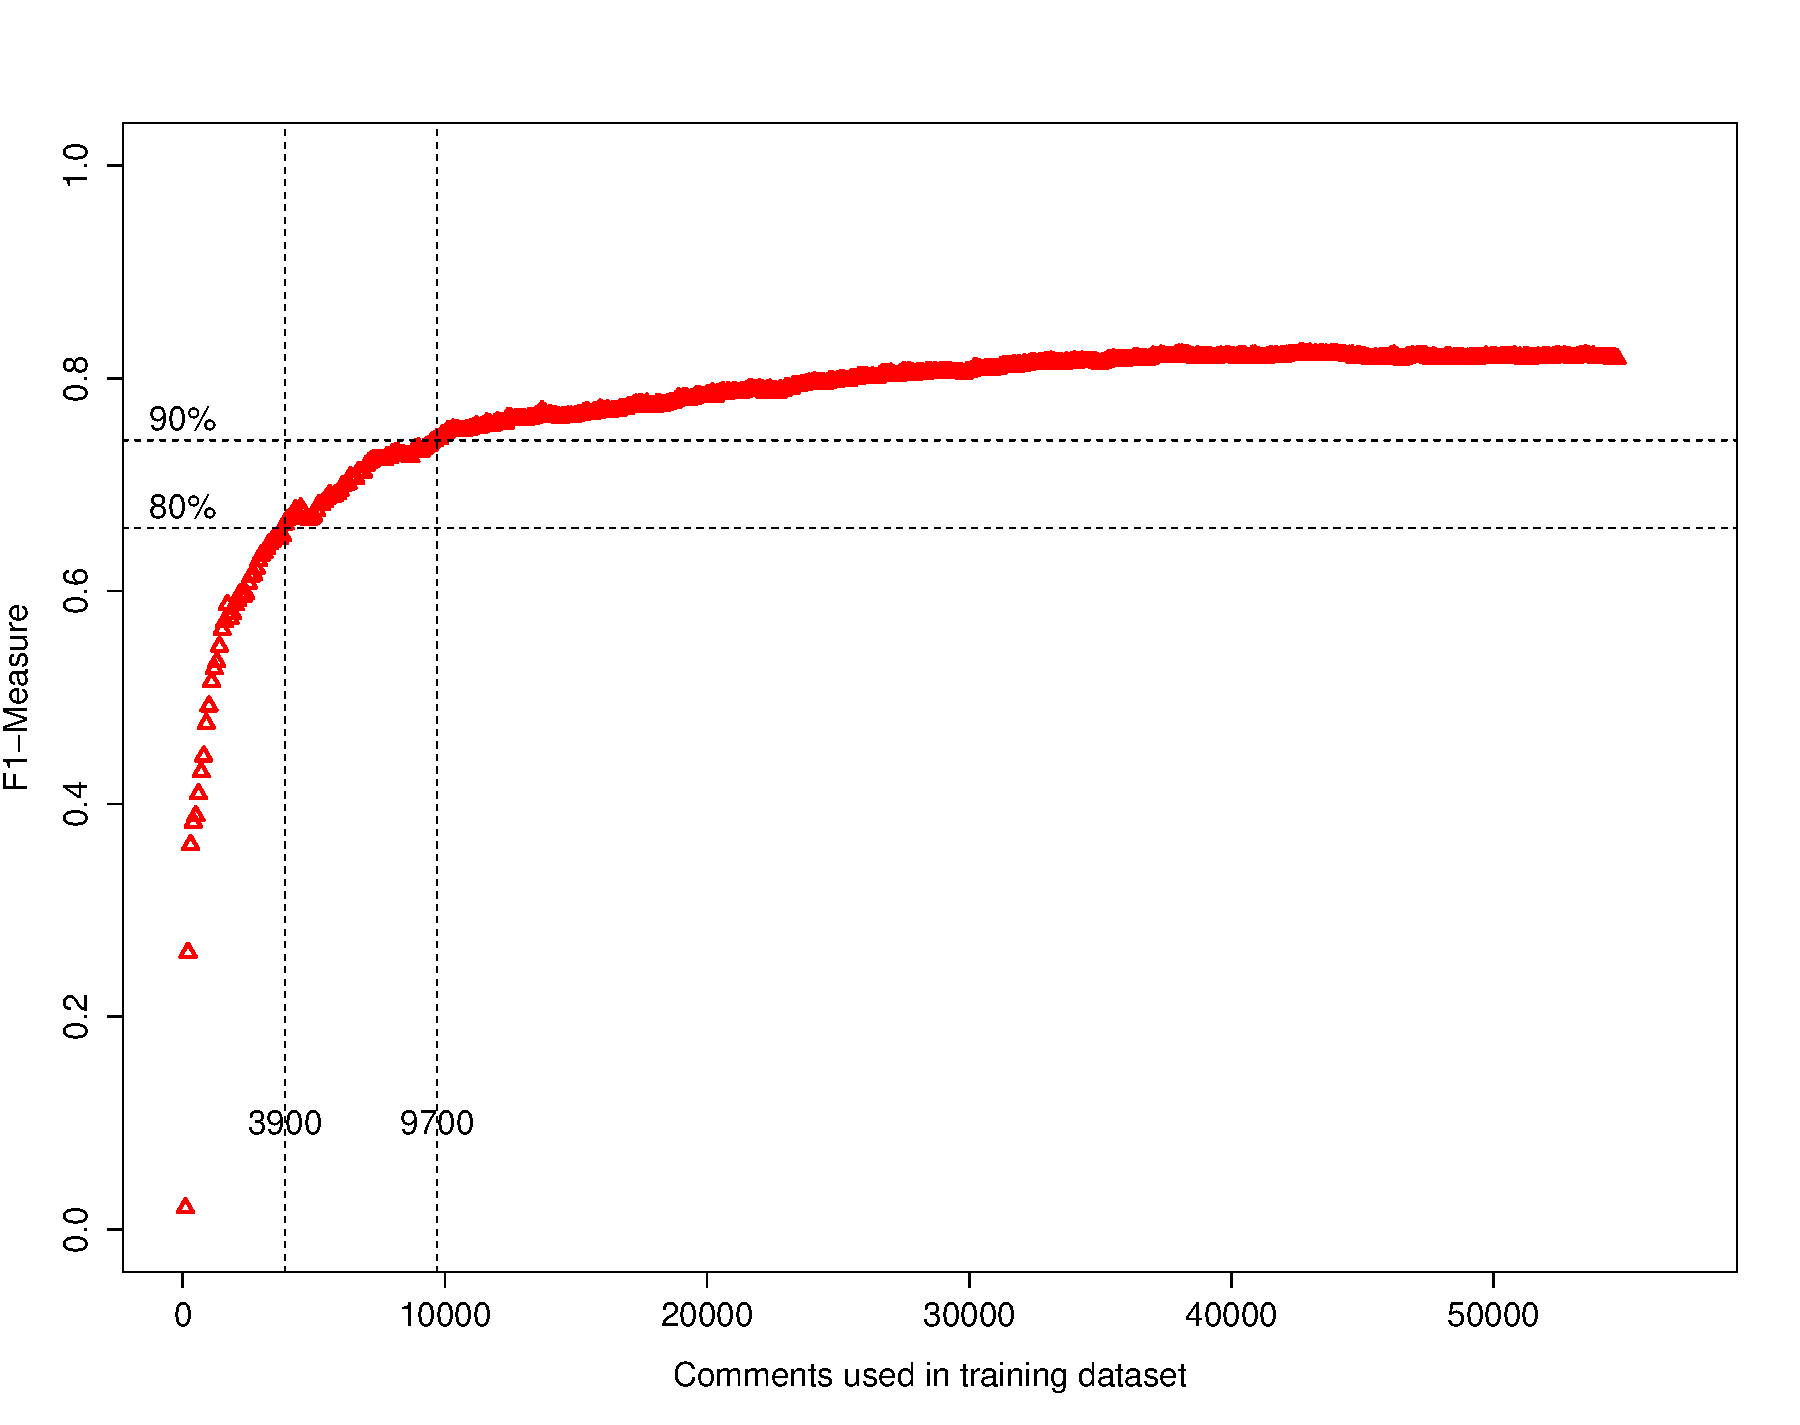
\includegraphics[width=0.49\textwidth]{figures/appendix/ten_fold_validation_design/ten_fold_validation_average_100.pdf}
    \label{fig:design_debt_per_comment_average}}
    \subfigure[Requirement Debt]{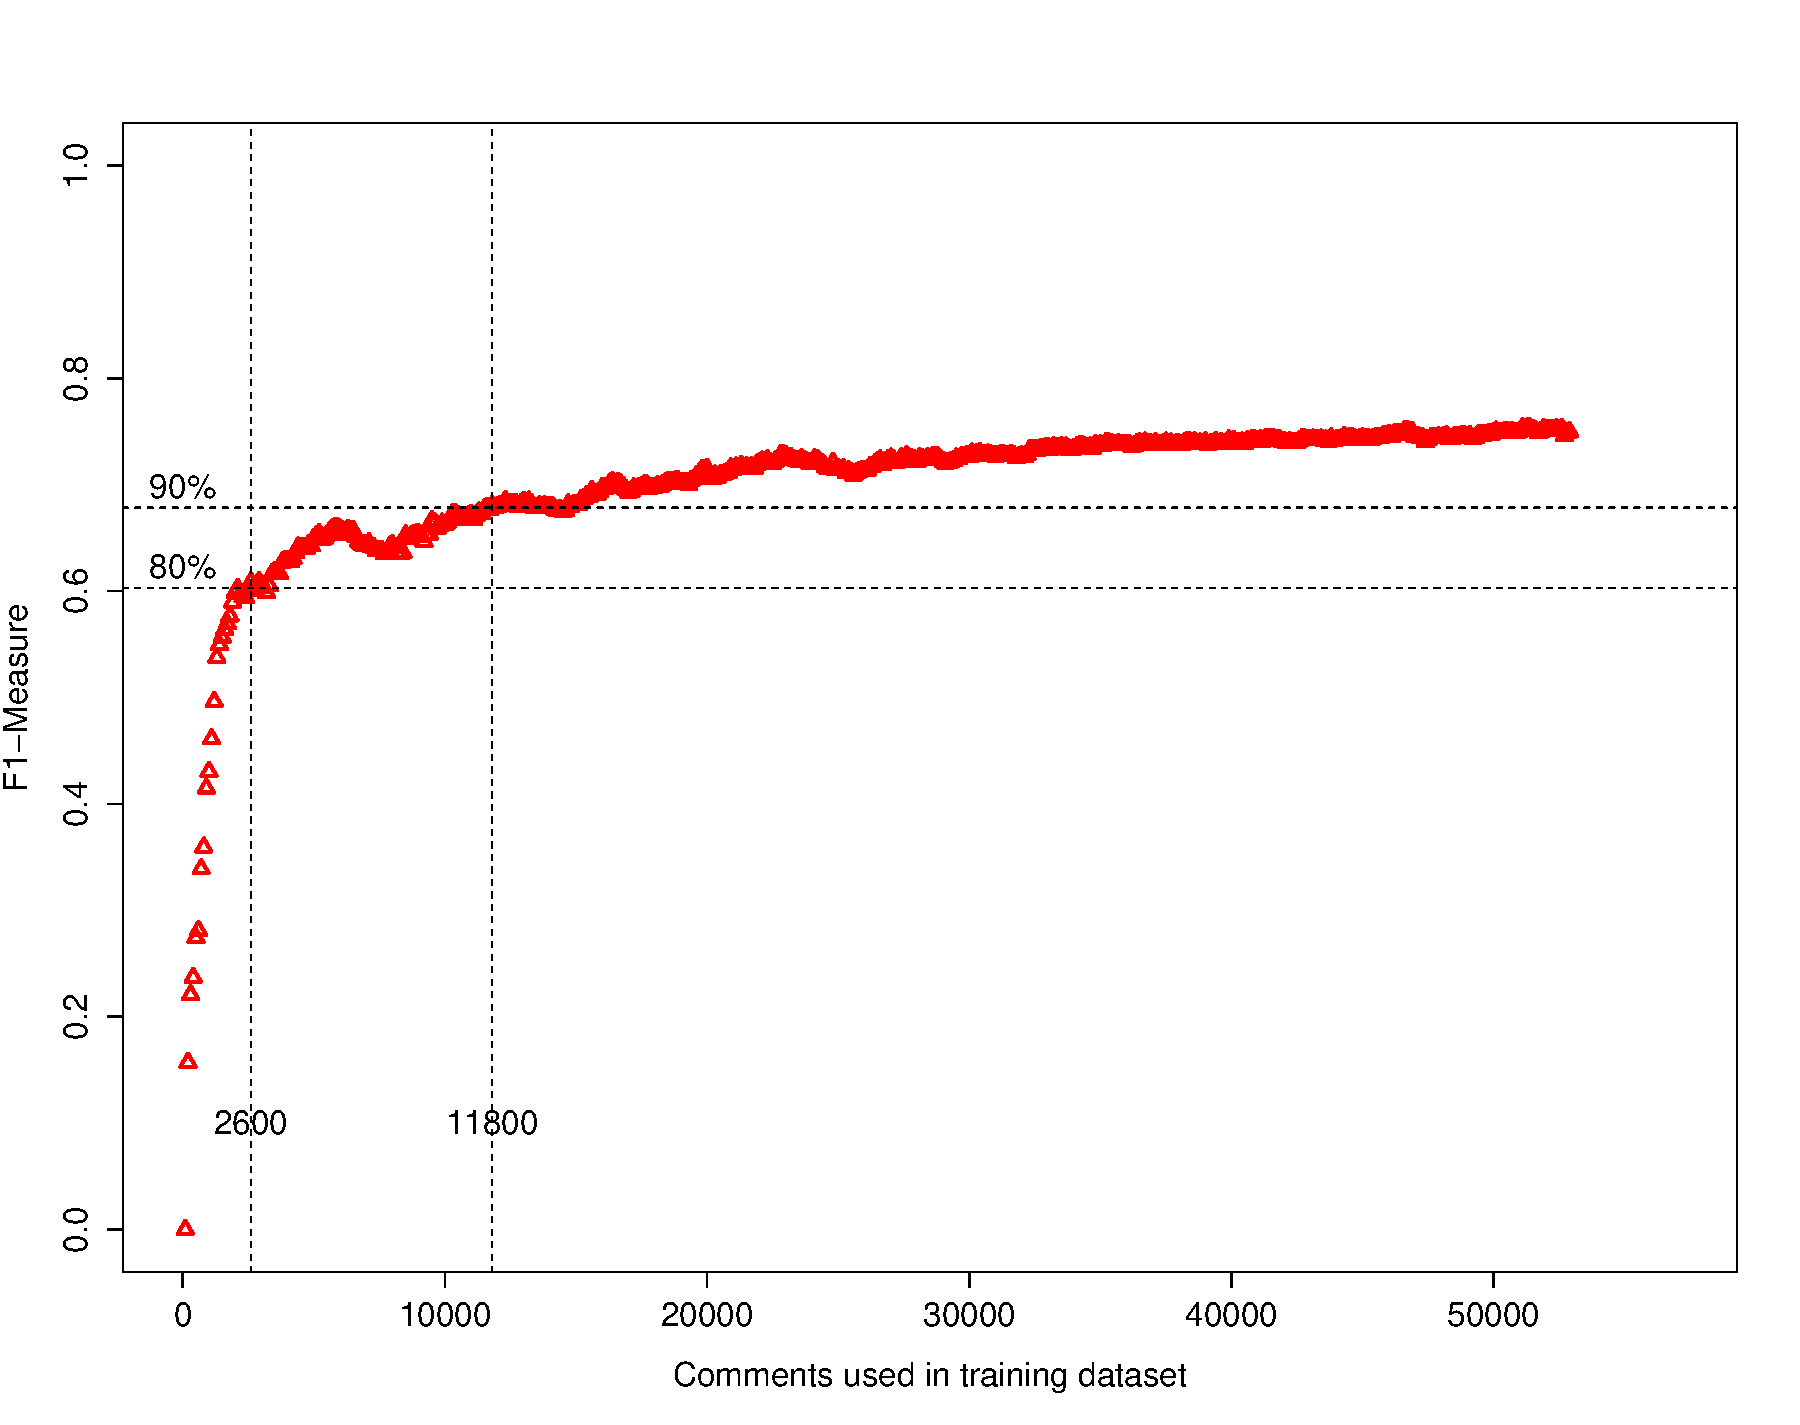
\includegraphics[width=0.49\textwidth]{figures/appendix/ten_fold_validation_requirement/ten_fold_validation_average_100.pdf}
    \label{fig:requirement_debt_per_comment_average}}
    \caption{F1-measure Achieved per Iteration (Per-comment base) }
\end{figure*}


\revised{\noindent \textbf{Per-comment based experiment results - design debt:} Figure~\ref{fig:design_debt_per_comment_average} shows the ten fold average F1-measure obtained while identifying design \SATD. We find that the maximum F1-measure improves as we increase the number of comments in the training dataset, achieving its highest value (i.e., 0.824) with 42,700 comments. However, the most accentuated improvement in the F1-measure performance happens within the first 10k comments, more precisely 80\% and 90\% of the maximum F1-measure is achieved with 3,900 and 9,700 comments in the training dataset. In this experiment we added 100 comments per iteration, and for each batch of 100 comments we keep the same ratio between design \SATD and without technical debt comments of the training dataset which is approximately 5\% (i.e., $\frac{2,703}{58,122}$). Therefore, we used 195 and 485 design \SATD comments to achieve 80\% and 90\% of the maximum F1-measure respectively. This amounts to a reduction of 90.86\% and 77.28\% in training data to achieve 80\% and 90\% of the maximum F1-measure.

The number of design \SATD comments needed to achieve 80\% and 90\% of the maximum F1-measure in our second experiment is considerable lower than the number of \SATD comments necessary to achieve similar marks on the first experiment. One possible reason is that in the second experiment (i.e., per-comment based) comments that belongs to same project are used as training data for the maximum entropy classifier.}{R2-14}

\revised{\noindent \textbf{Per-project based experiment results - requirement debt:}}{R2-14} We find that, although there is a variation in the F1-measure value during the first 3 iterations, they are not as preeminent as the variation found in design \SATD analysis. The F1-measure in requirement \SATD tends to be more constant through the iterations, and the first iteration has a high percentage of the maximum F1-measure achieved for each project. This shows that the way developers indicate requirement debt does not vary between different application domains as much as in design debt. This uniformity in requirement \SATD comments allows a good classification even with a small number of comments in the training dataset. We elaborate more on this point later in Section~\ref{sec:discussion}.

Figure \ref{fig:implementation_argo_result} shows the F1-measure for different iterations in ArgoUML. The highest F1-measure of 0.65 is achieved in the third iteration. From Figure~\ref{fig:implementation_argo_result}, we observe that we achieve more than 80\% of the highest F1-measure in the first iteration and more than 90\% in the second and subsequents iterations. The reduction in comments is 28.64\% and 62.31\% for the 90\% and 80\% of the maximum F1-measure, respectively.

Table \ref{tbl:requirement_iteration_performance} shows the average percentage of the maximum F1-measure for each iteration. Unlike the case of design debt, for requirement debt, the best F1-measure is achieved in the first iteration. This shows that using as few as 380 comments, we can effectively detect requirement \SATD\revised{as we can also see from Figure~\ref{fig:requirement_percentage_f1_measure}.}{R3-9}.

\begin{table}[!thb]
    \begin{center}
        \caption{Average Maximum F1-measure for Design Debt for All Projects}
        \label{tbl:design_iteration_performance}
        \begin{tabular}{l| c c c}
        \toprule
        \textbf{\thead{Iteration\\Number}} & \textbf{\thead{Average\%\\of maximum\\F1-measure}} & \textbf{\thead{$\Delta$\\between\\iterations}} & \textbf{\thead{Average\\comments}} \\ 
        \midrule
         \textbf{1}  &  0.718 &  -      & 756   \\  
         \textbf{2}  &  0.856 & 0.138   & 1,106 \\  
         \textbf{3}  &  0.924 & 0.068   & 1,444 \\  
         \textbf{4}  &  0.912 & -0.012  & 1,717 \\  
         \textbf{5}  &  0.927 & 0.016   & 1,919 \\  
         \textbf{6}  &  0.930 & 0.002   & 2,108 \\  
         \textbf{7}  &  0.963 & 0.029   & 2,251 \\  
         \textbf{8}  &  0.965 & 0.006   & 2,353 \\  
         \textbf{9}  &  0.959 & -0.002  & 2,432 \\  
        \bottomrule
        \end{tabular}
    \end{center}    
\end{table}

\begin{table}[!thb]
	\begin{center}
		\caption{Average Maximum F1-measure for Requirement Debt for All Projects}
		\label{tbl:requirement_iteration_performance}
		\begin{tabular}{l| c c c}
			\toprule
			\textbf{\thead{Iteration\\Number}} & \textbf{\thead{Average\%\\of maximum\\F1-measure}} & \textbf{\thead{$\Delta$\\between\\iterations}} & \textbf{\thead{Average\\comments}} \\
			\midrule
			\textbf{1}  &  0.873 &   -      &  380  \\  
	        \textbf{2}  &  0.772 & -0.101   &  481  \\
	        \textbf{3}  &  0.778 & 0.006    &  541  \\  
	        \textbf{4}  &  0.806 & 0.028    &  588  \\
	        \textbf{5}  &  0.795 & -0.011   &  620  \\
	        \textbf{6}  &  0.819 & 0.024    &  638  \\
			\textbf{7}  &  0.837 & 0.018    &  654  \\  
	        \textbf{8}  &  0.833 & -0.004   &  668  \\  
	        \textbf{9}  &  0.805 & -0.028   &  681  \\  
			\bottomrule
		\end{tabular}
	\end{center}    
\end{table}

\revised{\noindent \textbf{Per-comment based experiment results - requirement debt:} Figure~\ref{fig:requirement_debt_per_comment_average} shows the ten fold average F1-measure obtained while identifying requirement \SATD. As intuitively expected, the F1-measure increases as we add more data into the training dataset, and again the biggest improvement happens around the first 10k of comments. For requirement \SATD we achieved 80\% of the maximum F1-measure using 2,600 comments and 90\% of the maximum F1-measure with 11,800. During this experiment we increase the size of the training dataset 100 comments per time, and within each batch of 100 comments we added 2 requirement \SATD comments to keep the same approximate ratio of the total requirement \SATD and without technical debt comments (i.e., $\frac{757}{58,122}$) until we have added all requirement \SATD comments available to train. While training the dataset with 2,600 comments (80\% of the maximum F1-measure) we are in fact adding 52 requirement \SATD comments, whereas to achieve 90\% of the maximum F1-measure we used 236 requirement \SATD comments. The maximum F1-measure achieved was 0.753 using 51,300 comments of which 675 were requirement \SATD, and therefore, this amounts to a reduction of 92.29\% and 65.03\% in training data to achieve 80\% and 90\% of the maximum F1-measure.}{R2-14}
  
The results of this RQ show that, contrary to our initial intuition, more data may not always result in higher classification accuracy. In fact, we find that in some cases, the addition of more comments can decrease the performance of the classifier. One of the reasons for this is that the weight of features is given through empirical probability, and consequently features that appear more will have a higher weight. Although this is an effective process for the majority of the cases we studied, it can be misleading when classifying comments that have different contexts, i.e., in cross-project classification.

\conclusionbox{We find that using our NLP-based approach, design \SATD comments can be classified effectively using a training dataset of 1,106 - 1,444 comments. Similarly, requirement \SATD can be classified with as little as 380 comments of this type.}